% Keck DSST section

For long, we believed that telluric contamination was the major culprit
behind the \keck\ RV-BC anomaly. However, the simulations in previous
section have revealed that tellurics probably only contribute a small
amount, mostly buried underneath photon noise and algorithmic
errors. We quickly focused our suspicion to DSST, because we saw the
differences in DSSTs before and after telluric cleaning (described in
Section~\ref{keck:telluric:real}), which are often larger than the
micro-telluric lines and could easily manifest as trends in the RV-BC
plane.

Any errors in the DSST, i.e., differences between the true stellar
spectrum and our assumed knowledge of truth (the DSST), are just like
persisting spectral contamination in the star's frame (instead of the
Earth's frame like the telluric contamination). Therefore, it beats
against the iodine lines as the stellar lines move back and forth
through the forest of iodine lines due to the Earth barycentric motion
and the star's intrinsic RV variation. As a result, it manifests as
anomalous RV-BC trends and adds bias and scatter to the final RVs.

We do know for sure that there are errors in the DSST, but the
question is how much, and more importantly, how much do these errors
translate into RV errors.


%----------------------------------------------------------------
% Effect of imperfect DSST
% plot made by ~/Exo.../Keck.../simulate.../msplot.pro, plot_name='3panel'
\begin{figure}
\subfloat[HD 185144]{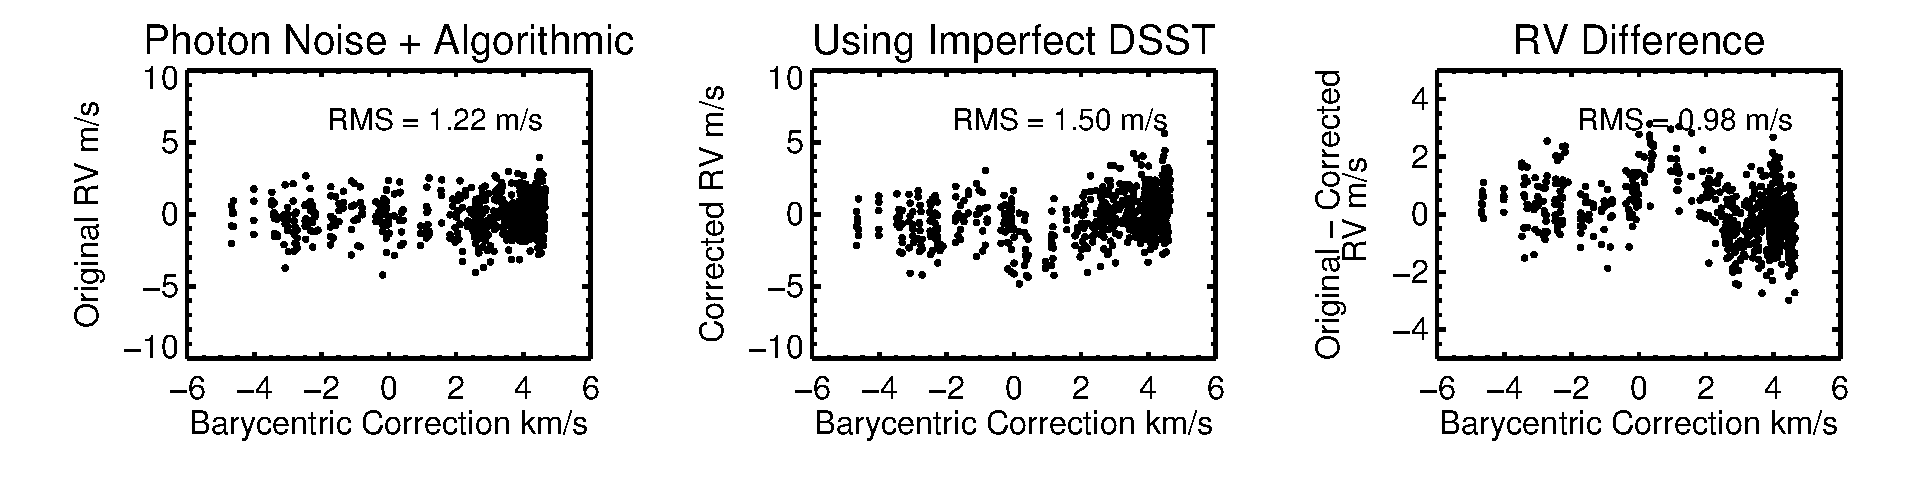
\includegraphics[scale=0.42]{keck/185144-rv-bc-3panel-test0-testd0.eps}}\
\subfloat[HD 10700]{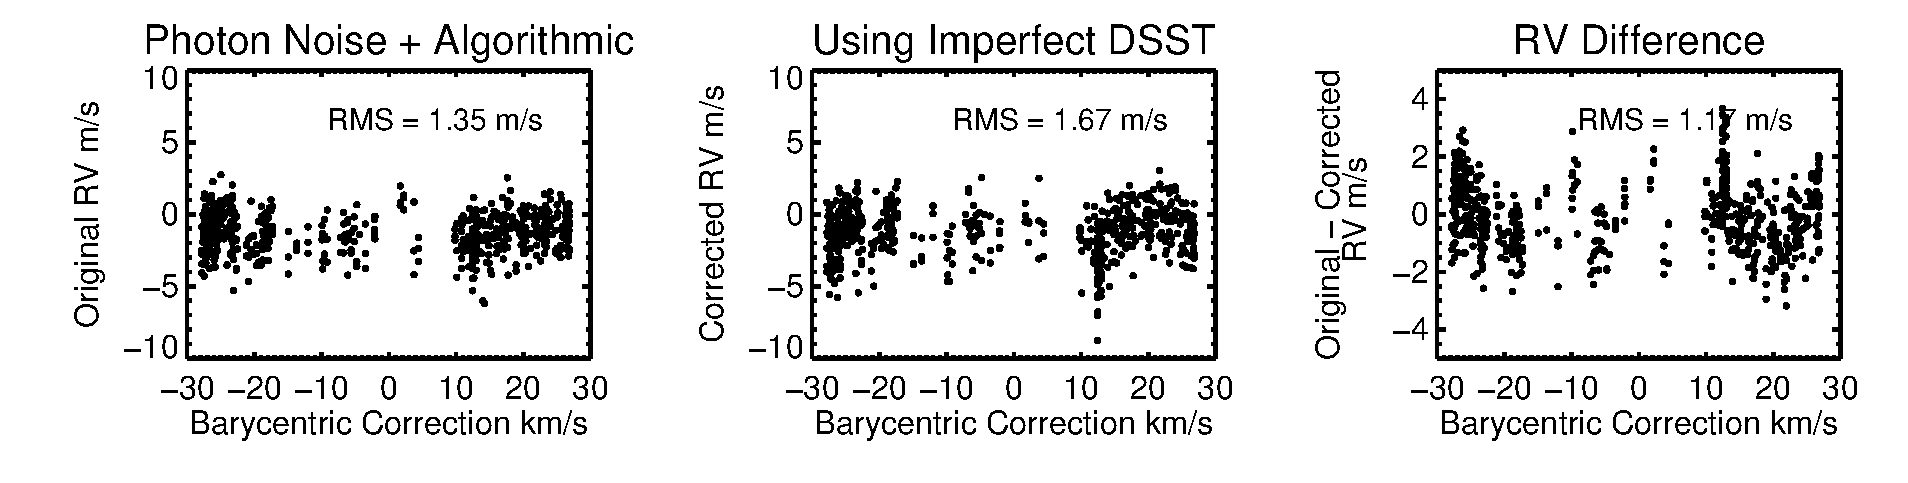
\includegraphics[scale=0.42]{keck/10700-rv-bc-3panel-test0-testd0.eps}}\
\caption{Effect of imperfect DSST on simulated data.
\label{keck:fig:dsst}}
\end{figure}
%----------------------------------------------------------------


%----------------------------------------------------------------
% Chunk illustration of effect of imperfect DSST
% plot made by ~/Exo.../Keck.../simulate.../msplot.pro, plot_name='makefakedsst','chunkcomp'
\begin{figure}
\subfloat{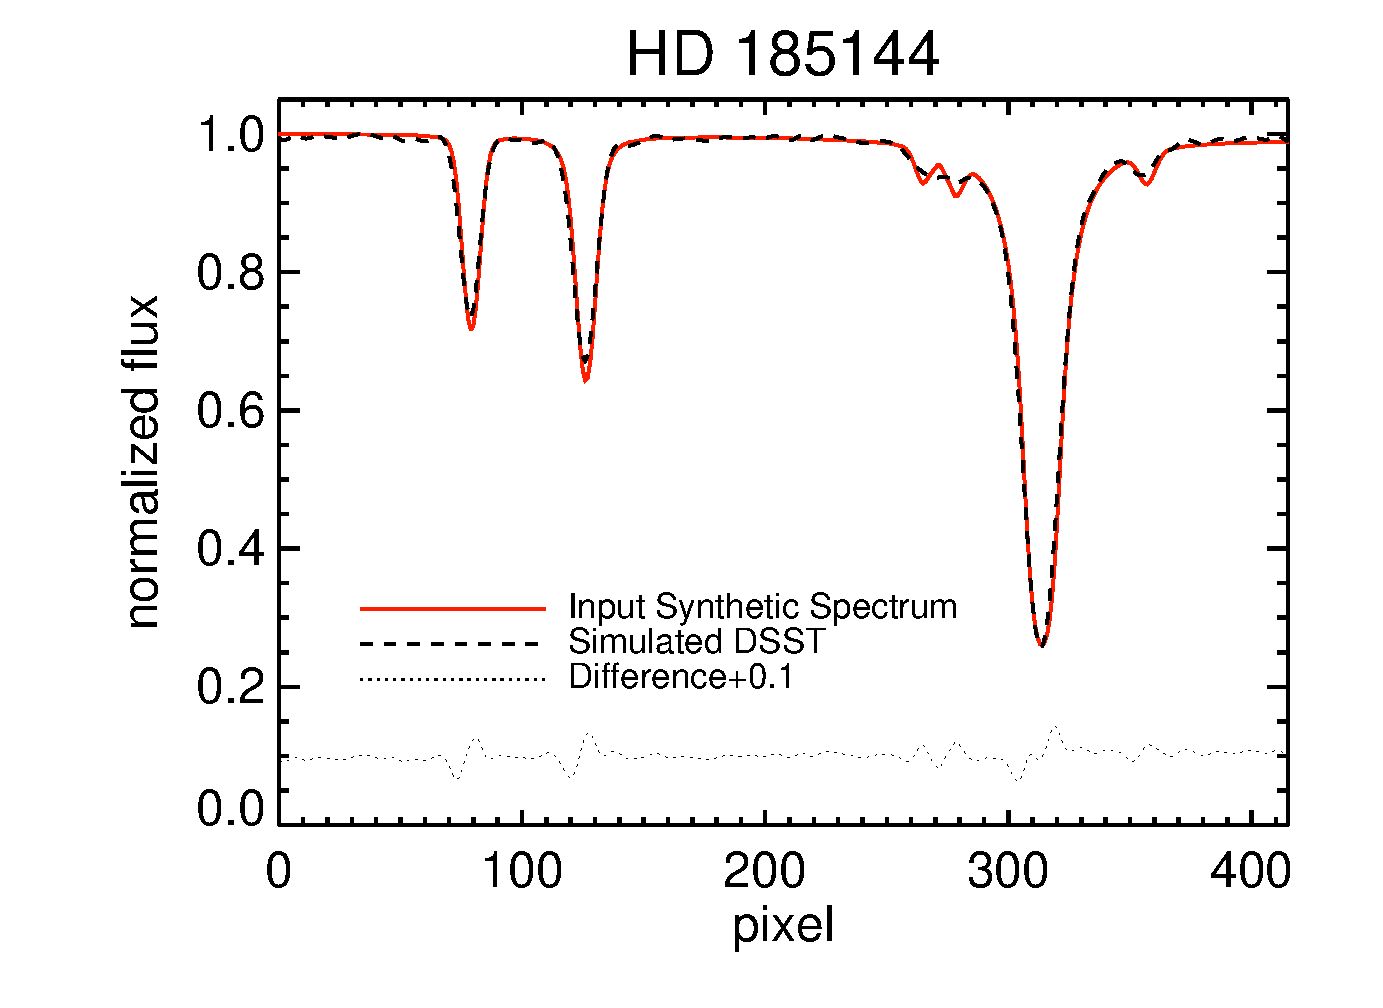
\includegraphics[scale=0.3]{keck/185144_makefakedsst_100.eps}}
\subfloat{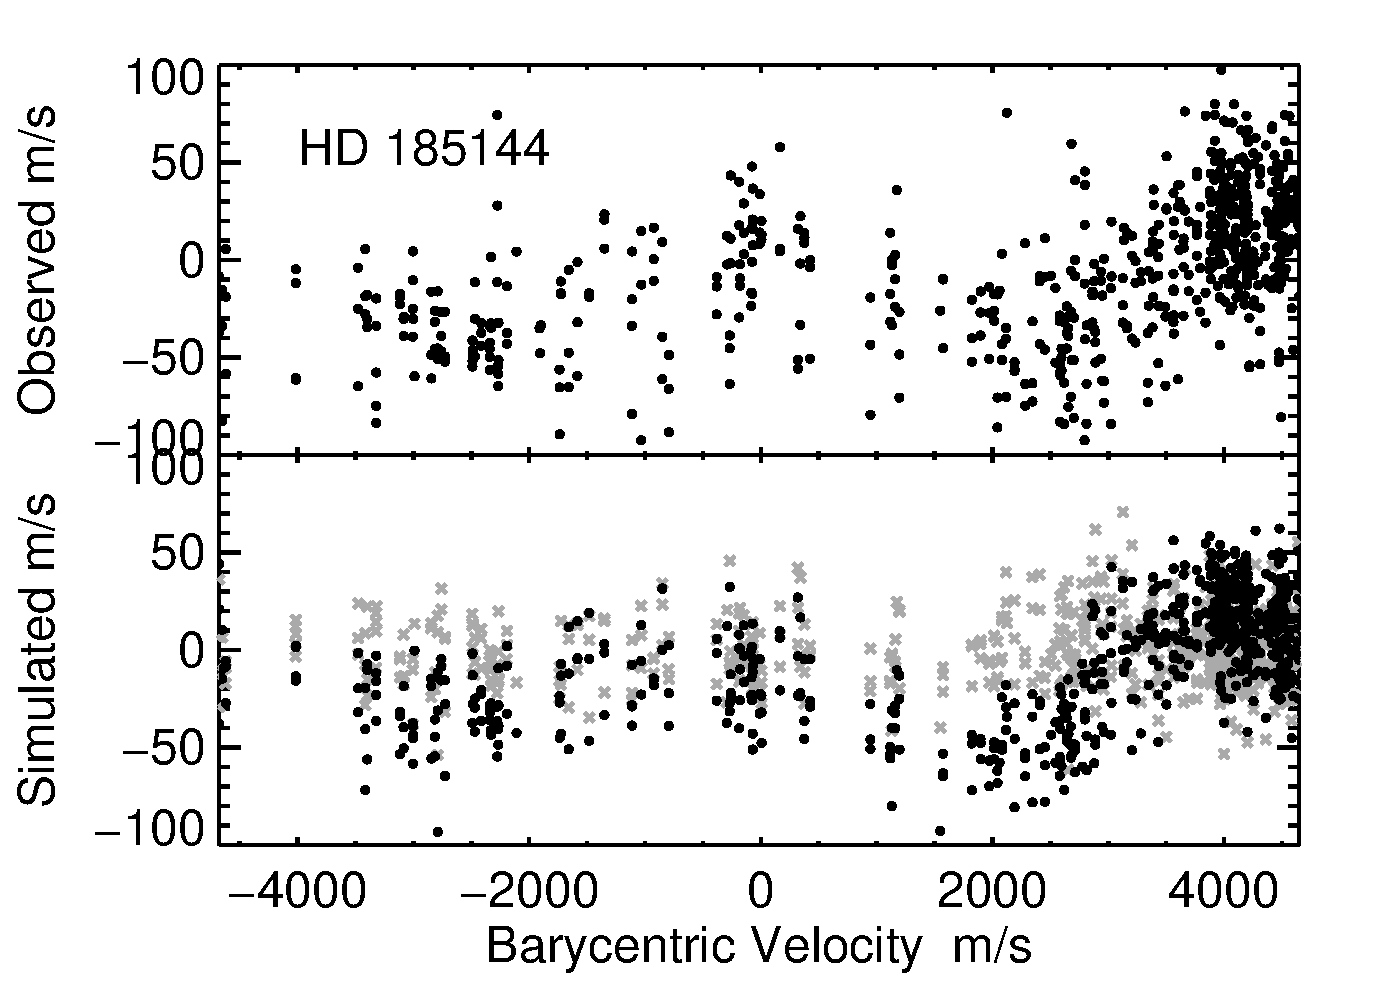
\includegraphics[scale=0.3]{keck/185144_chunkcomp_100.eps}}\
\subfloat{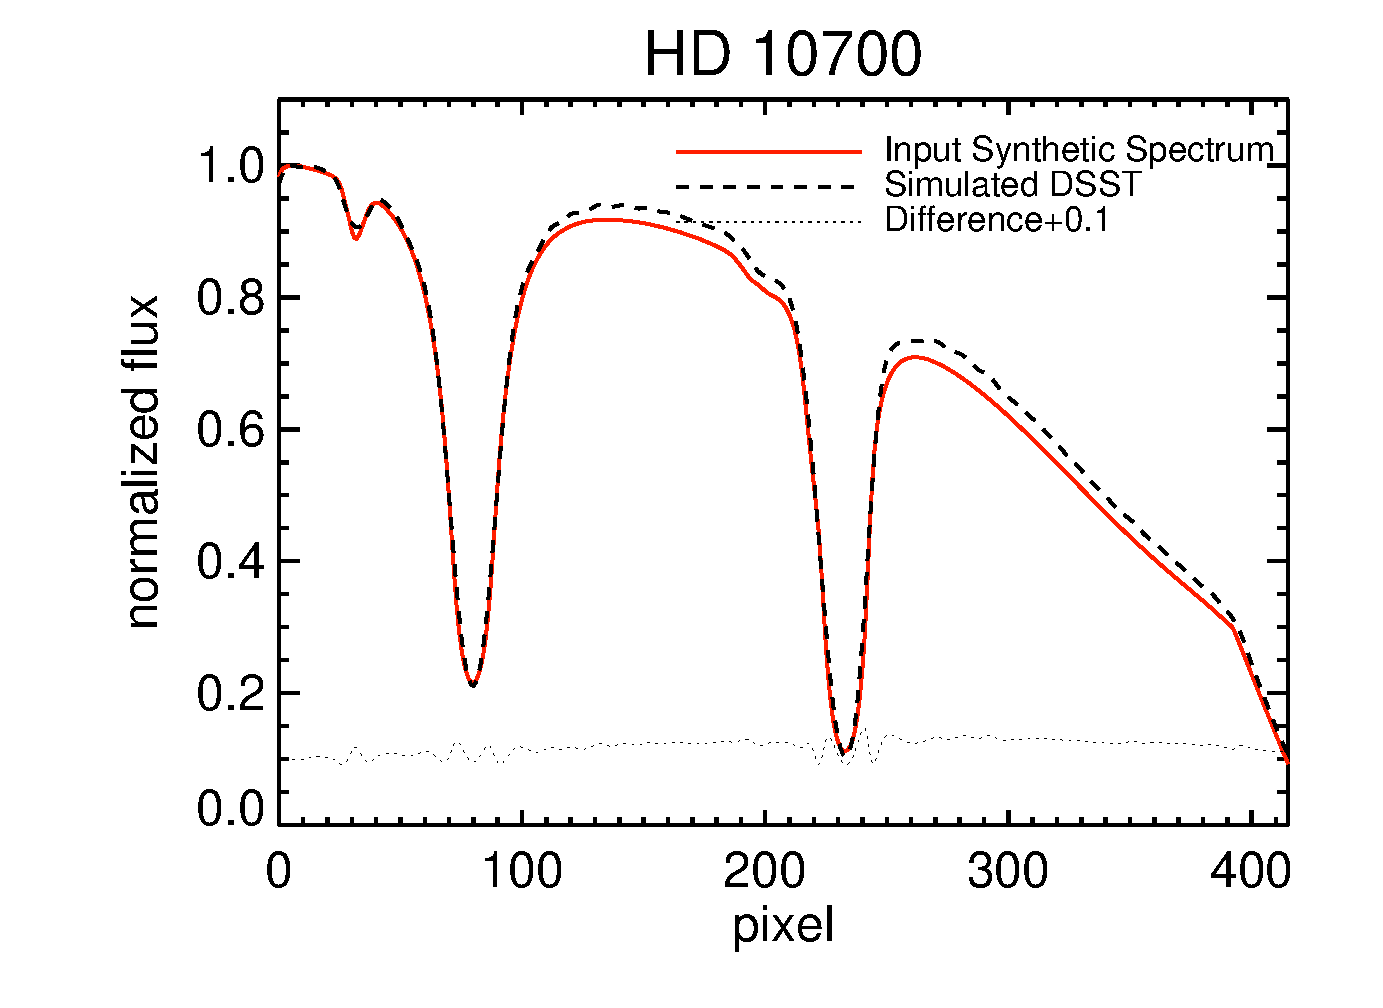
\includegraphics[scale=0.3]{keck/10700_makefakedsst_104.eps}}
\subfloat{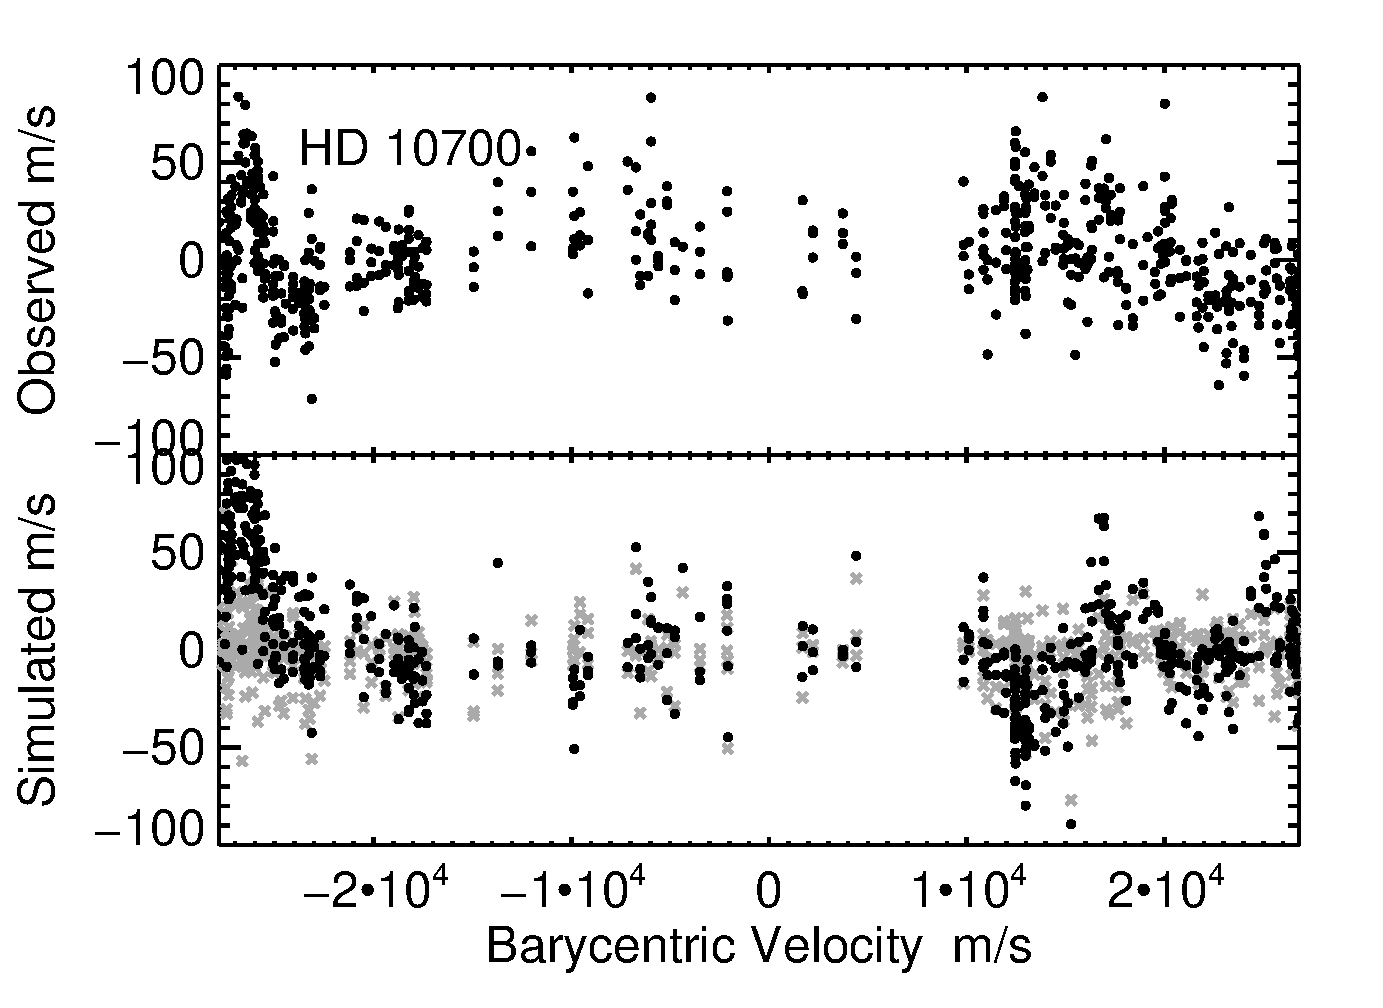
\includegraphics[scale=0.3]{keck/10700_chunkcomp_104.eps}}\
\caption{Effect of imperfect DSST on simulated data for a single
spectral chunk. HD 185144 is for a chunk near 5160\AA, and HD 10700 is
for a chunk around 5166\AA, which are spectral regions that tend to
receive high weights due to ample stellar lines and a lack of telluric
lines.
\label{keck:fig:dsstchunk}}
\end{figure}
%----------------------------------------------------------------

